\documentclass[a4paper,12pt]{article}
\usepackage[english]{babel}
\usepackage[utf8]{inputenc}

%
% For alternative styles, see the biblatex manual:
% http://mirrors.ctan.org/macros/latex/contrib/biblatex/doc/biblatex.pdf
%
% The 'verbose' family of styles produces full citations in footnotes, 
% with and a variety of options for ibidem abbreviations.
%
\usepackage{graphicx}
\usepackage{csquotes}
\usepackage[style=verbose-ibid,backend=bibtex]{biblatex}
\bibliography{sample}

\usepackage{lipsum} % for dummy text

\title{A Distributional Perspective on Reinforcement Learning}

\author{Shayan Amani}

\date{\today}

\begin{document}
\maketitle

% \section{Introduction}
This paper proposes distributional Bellman optimality operator on which later they discuss an algorithm, namely Approximate Distributional Learning. The mentioned algorithm includes evaluation and control steps. 

 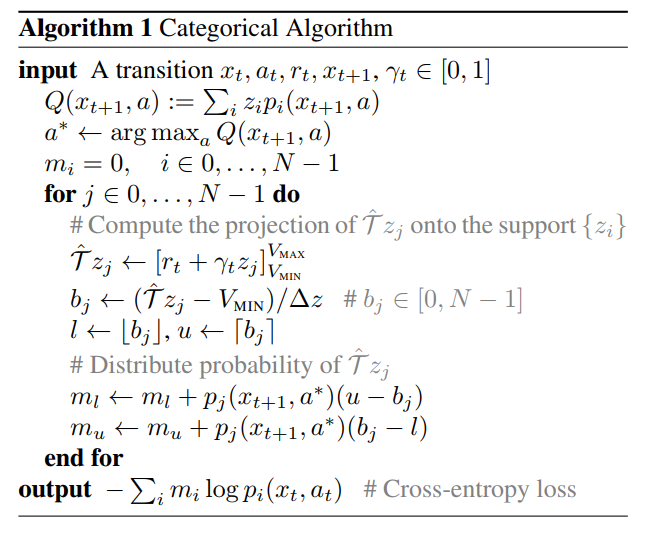
\includegraphics[width=1\columnwidth]{alg1.png}


The Authors attempted to emphasize on the importance of considering value distribution than the expectation of this distribution, so called \textit{value}. This paper is like a new approach to reinforcement learning problems like what DeepMind's paper done with Deep Q-Network (DQN).





% This is an example citation \autocite{ginsberg}.
% \lipsum[1] % dummy text

% This is another example citation \autocite{brassard}.
% \lipsum[2] % dummy text

% This is a repeated citation \autocite{brassard}.
% \lipsum[3] % dummy text

% This is another example citation \autocite{adorf}.
% \lipsum[4] % dummy text 

\end{document}